\begin{figure}[ht!]
  \centering
\begin{subfigure}{.5\linewidth}
\centering
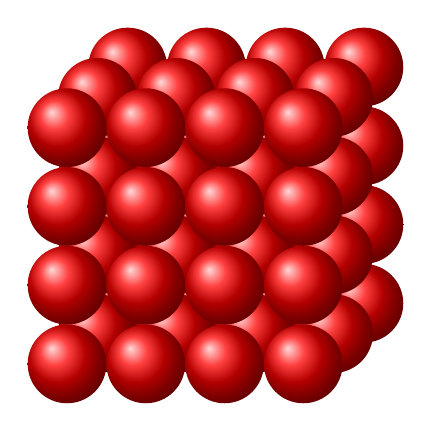
\begin{tikzpicture}
  \foreach \z in {1,2,3}{
  \foreach \i in {3,2,1,0}{% This one doesn't matter
    \foreach \j in {3,2,1,0}{% This will crate a membrane
        \shade[ball color=red] ({\i},{\j},\z) circle(0.5);
      }
    }
  }
\end{tikzpicture}
\subcaption{} \label{fig:M1}
\end{subfigure}%
\par\bigskip

\begin{subfigure}{1.0\linewidth}
\centering
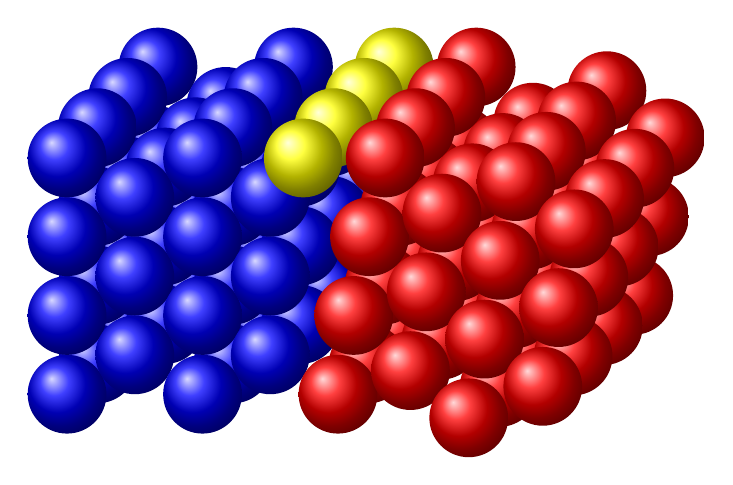
\begin{tikzpicture}
    \foreach \x in {0,1,2,3}{%
      \foreach \z in {0,1,2,3}{%
      \shade[ball color=blue] (0,\x,\z) circle(0.5);
      }
    }
    \foreach \x in {0.5,1.5,2.5}{%
      \foreach \z in {0,1,2,3}{%
      \shade[ball color=blue] ({1*sqrt(0.74)},\x,\z) circle(0.5);
      }
    }
    \foreach \x in {0,1,2,3}{%
      \foreach \z in {0,1,2,3}{%
      \shade[ball color=blue] ({2*sqrt(0.74)},\x,\z) circle(0.5);
      }
    }
    \foreach \x in {0.5,1.5,2.5}{%
      \foreach \z in {0,1,2,3}{%
      \shade[ball color=blue] ({3*sqrt(0.74)},\x,\z) circle(0.5);
      }
    }
    \foreach \z in {0,1,2,3}{%
      \shade[ball color=yellow] ({3},3,\z) circle(0.5);
    }
    \foreach \y in {0,1,2,3}{%
      \foreach \z in {0,1,2,3}{%
      \shade[ball color=red] ({4*sqrt(0.74)+0.2*\y},\y,\z) circle(0.5);
      }
    }
    \foreach \y in {0.3,1.3,2.3}{%
      \foreach \z in {0,1,2,3}{%
      \shade[ball color=red] ({5*sqrt(0.74)+0.2*\y},\y,\z) circle(0.5);
      }
    }
    \foreach \y in {-0.3,0.7,1.7,2.7}{%
      \foreach \z in {0,1,2,3}{%
      \shade[ball color=red] ({6*sqrt(0.74)+0.2*\y},\y,\z) circle(0.5);
      }
    }
    \foreach \y in {0.1,1.1,2.1}{%
      \foreach \z in {0,1,2,3}{%
      \shade[ball color=red] ({7*sqrt(0.74)+0.2*\y},\y,\z) circle(0.5);
      }
    }


\end{tikzpicture}
\subcaption{} \label{fig:M2}
\end{subfigure}%
\par\bigskip

\begin{subfigure}{1.0\linewidth}
\centering
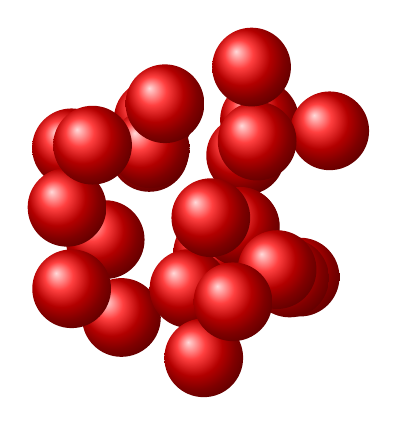
\begin{tikzpicture}
  \foreach \z in {0,...,24}{
    \shade[ball color=red] ({rand*1.5},{rand*1.5},{rand*1.5}) circle(0.5);
  }
\end{tikzpicture}
\subcaption{} \label{fig:M3}
\end{subfigure}
\par\bigskip
\caption{Schematic representation of different degrees of ordered structures, where (a) is a crystalline of a simple cubic lattice, (b) is a polycrystalline of a hexagonal lattice, and (c) is an amorphous. }
\label{fig:crystalstructure}
\end{figure}
